\documentclass[aspectratio=169]{beamer}
\usepackage{listings}
\usepackage{luatexja}
\usepackage{graphicx}
\usepackage{tikz}
\usepackage{hyperref}

\hypersetup{
  colorlinks=true,
  pdftitle={Pythonと東海と私}}

\title{Pythonと東海と私}
\author{Atsushi Odagiri}
\date{2024-11-16}
\begin{document}

\section{はじめに}
\begin{frame}
\titlepage
\end{frame}

\begin{frame}
\frametitle{Agenda}
\tableofcontents
\end{frame}

\begin{frame}
\frametitle{お前誰よ}
\begin{columns}
\begin{column}{0.47\linewidth}
\begin{itemize}
\item Atsushi Odagiri
\item 2000年〜2004年 豊橋技術科学大学
\item 2005年 名古屋で就職
\item 2016年〜 Open Collector
\item Pythonは大学時代に1.5くらいのころから
\end{itemize}
\end{column}
\begin{column}{0.47\linewidth}
\begin{figure}[h]

\includegraphics[width=\linewidth]{oc-logo.png}
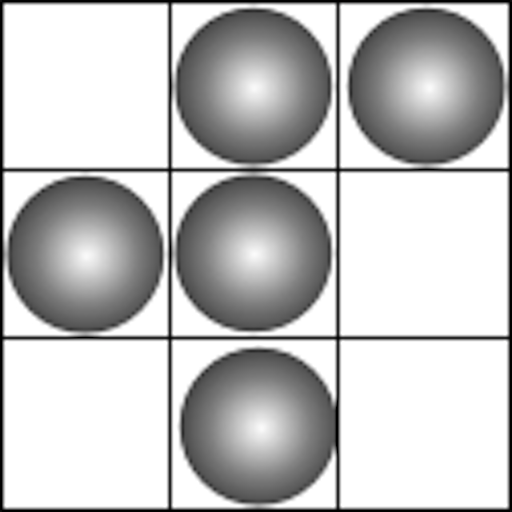
\includegraphics[width=0.47\linewidth]{r-penta512.png}

\includegraphics[width=0.47\linewidth]{kenall.png}
\end{figure}
\end{column}
\end{columns}
\end{frame}

\section{Pythonと私}
\begin{frame}
\frametitle{Pythonと私}
\begin{itemize}
\item aodag青春グラフィティ後半 東海編
\item 前半の静岡編はPyCon mini 静岡でやる予定だったのにね(´・ω・`)
\end{itemize}
\end{frame}

\begin{frame}
\frametitle{2000年 ハッカーになろう}

\begin{itemize}
\item 当時豊橋の大学生
\item How To Become A Hacker (和訳:ハッカーになろう) を読んでPythonに触れる
\begin{itemize}
\item 当時のバージョンでは学ぶべき言語は Python, Perl, C, Lisp となっていた
\item 後のバージョンでJavaが加わりGoにも言及している
\end{itemize}
\end{itemize}

\end{frame}

\begin{frame}
\frametitle{2001年 - 2002年 Zopeとかコミュニティとか}
\begin{itemize}
\item 当時PythonといえばZopeという勢いがあった
\item Japan Zope Users Group(JZUG)
\item 名古屋のコミュニティ参加
\item Nagoya Zope Users Group(NZUG)
\end{itemize}
\end{frame}

\begin{frame}
\frametitle{2004年 - 2005年 就職と秘密兵器}
\begin{itemize}
\item 名古屋で就職
\item Pythonの仕事?ありません
\item JavaとかPHP、あと .NET
\item こっそりインストールしたPythonでデータ生成やテキスト加工とかこっそりやる
\begin{itemize}
\item スクリプトとして正しい使い方
\end{itemize}
\end{itemize}
\end{frame}

\begin{frame}
\frametitle{2006年 Pythonコミュニティへ}
\begin{itemize}
\item 一回目の転職もこのころ
\item Python Developers Camp 2006 富士
\item その年忘年会を各地で同時開催 名古屋で幹事をやる
\end{itemize}
\end{frame}

\begin{frame}
\frametitle{2007年 東海 Python Workshop}
\begin{itemize}
\item Python Developers Camp 2007 Winter 志賀高原
\item 東海 Python Workshop 01
\begin{itemize}
\item 30人くらいは来てくれた記憶
\item 地元発表者の不足
\item 地元コミュニティが必要だ
\end{itemize}
\end{itemize}
\end{frame}

\begin{frame}
\frametitle{2008年 Python東海}
\begin{itemize}
\item 2008年に開始した...と思う
\item 割とすぐに東京に行くことになってしまい、早々に主催を交代
\item 主催はどんどん変わっていいです
\end{itemize}
\end{frame}

\begin{frame}
\frametitle{名古屋で勉強会とか}
\begin{itemize}
\item FLOSS桜山
\item メンバーがかぶりがちな勉強会主催者がよく来るので日程調節
\end{itemize}
\end{frame}

\section{Python Packaging}

\begin{frame}
\frametitle{Pythonパッケージングのおさらいをしよう}
\begin{large}
pythonパッケージをインストールしてみましょう
\end{large}
\end{frame}

\begin{frame}
\frametitle{Pythonパッケージをインストール}
\begin{itemize}
\item Python Packaging はPEPで定義されるようになっています
\item PEPとPython本体の仕様だけを信じてインストールしてみましょう
\item pythonで実行するとうっかりpipを呼んでしまいそうなのでUNIXコマンドを使います
\end{itemize}
\end{frame}


\begin{frame}
\frametitle{パッケージをインストールして使えるまで}
\begin{itemize}
\item pypiで配布物のダウンロードURLを取得
\item 配布物をダウンロード
\item 配布物をインストール先に展開
\end{itemize}
\end{frame}

\begin{frame}
\frametitle{どこからダウンロードする?}
PEP 503, 691 にあります
\begin{itemize}
\item PyPIのprojectデータ
\item Simple Repository
\end{itemize}
\end{frame}

\begin{frame}[fragile]
PEP 503 にしたがってPyPIのプロジェクトデータを確認します。
\frametitle{Simple Repository}
\begin{itemize}
\item https://pypi.org/simple/{project}/ で情報を取得
\end{itemize}
\begin{lstlisting}
$ curl https://pypi.org/simple/pyramid/
\end{lstlisting}
HTMLが返ってきます。このHTMLをパースしてもよいのですが...
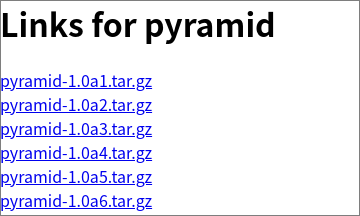
\includegraphics[width=0.3\linewidth]{pypi-pyramid.png}
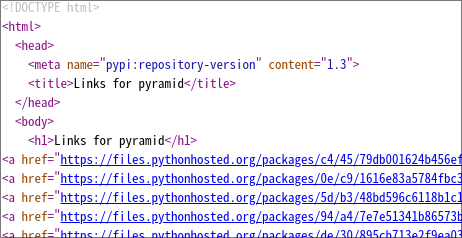
\includegraphics[width=0.3\linewidth]{pypi-pyramid-source.png}
\end{frame}

\begin{frame}[fragile]

\frametitle{JSON API}
PEP691 にはJSON APIが定義されていてACCEPTヘッダでレスポンスが変わることとなっています。

\begin{itemize}
\item https://pypi.org/simple/{project}/ で情報をJSONで取得
\item application/vnd.pypi.simple.v1+json ACCEPTヘッダでJSONを受け取る
\item 情報が多いのでファイル名だけjqで抜き取ってみます
\end{itemize}
\begin{lstlisting}
$ curl https://pypi.org/simple/pyramid/ \
    -H "ACCEPT: application/vnd.pypi.simple.v1+json" \
	| jq -c ".files[].filename"
\end{lstlisting}
\end{frame}


\begin{frame}[fragile]
\frametitle{PyPIから取得できた情報}
\begin{lstlisting}
"pyramid-1.0a1.tar.gz"
"pyramid-1.0a2.tar.gz"
...
"pyramid-2.0.1-py3-none-any.whl"
"pyramid-2.0.1.tar.gz"
"pyramid-2.0.2-py3-none-any.whl"
"pyramid-2.0.2.tar.gz"
\end{lstlisting}
いっぱいありますね
\end{frame}

\begin{frame}
\frametitle{どれをダウンロードしよう?}

例えば pyramid-2.0.2-py3-none-any.whl をPEP 427 にしたがって解釈すると以下のような情報が入っています。

\begin{itemize}
\item pyramid 配布物の名前
\item 2.0.2 配布物のバージョン
\item py3 対応しているpythonバージョン
\item none バイナリの形式
\item any プラットフォームOSやリンクしているlibcなどのアーキテクチャ
\item whl 配布物の形式
\end{itemize}
\end{frame}

\begin{frame}[fragile]
\frametitle{ダウンロード}
いったんは最新バージョンでwheelファイルをダウンロードしてみましょう。
\begin{lstlisting}
$ curl https://pypi.org/simple/pyramid/ \
    -H "ACCEPT: application/vnd.pypi.simple.v1+json" \
	| jq -c '.files[] 
	| select(
       .filename == "pyramid-2.0.2-py3-none-any.whl").url'
\end{lstlisting}
https://files.pythonhosted.org/packages/db/41/a[..]af/pyramid-2.0.2-py3-none-any.whl
\end{frame}

\begin{frame}
\frametitle{ダウンロードした配布物のフォーマット}
\begin{itemize}
\item sdist pyproject.toml を含むアーカイブ(zip, tar)ファイル
\item bdist wheel ソースコードとメタデータを含むZIPファイル
\end{itemize}

pyramid-2.0.2-py3-none-any.whl はwheelファイルフォーマットの配布物
\end{frame}

\begin{frame}[fragile]
\frametitle{wheelファイルの中身}
とりあえずZIPファイルなのでunzipで中を見てみましょう
\begin{lstlisting}
$ unzip -t pyramid-2.0.2-py3-none-any.whl
Archive:  pyramid-2.0.2-py3-none-any.whl
    testing: pyramid/__init__.py      OK
    testing: pyramid/asset.py         OK
    testing: pyramid/authentication.py   OK
	...
    testing: pyramid/scripts/ptweens.py   OK
    testing: pyramid/scripts/pviews.py   OK
    testing: pyramid-2.0.2.dist-info/LICENSE.txt   OK
    testing: pyramid-2.0.2.dist-info/METADATA   OK
    testing: pyramid-2.0.2.dist-info/WHEEL   OK
    testing: pyramid-2.0.2.dist-info/entry_points.txt   OK
    testing: pyramid-2.0.2.dist-info/top_level.txt   OK
    testing: pyramid-2.0.2.dist-info/RECORD   OK
\end{lstlisting}
\end{frame}

\begin{frame}
\frametitle{dist-info}
PEP427 によると {project}.dist-infoディレクトリにはソースコード以外の配布物の情報が入っている
\begin{itemize}
\item パッケージメタデータ METADATA
\item wheelに関する情報 WHEEL
\item インストールデータベース(要はファイル一覧) RECORD
\item ライセンスファイルやその他色々(setuptools由来のものとかまだ入ってる)
\end{itemize}
\end{frame}

\begin{frame}
\frametitle{パッケージメタデータを読む理由}
\begin{itemize}
\item パッケージメタデータから依存ライブラリの情報を取得
\begin{itemize}
\item 依存関係のグラフを作成してバージョン指定などを解決(難しいので今日は割愛)
\end{itemize}
\end{itemize}
\end{frame}

\begin{frame}[fragile]
\frametitle{さあインストールだ}
\begin{itemize}
\item どのディレクトリに?
\item site-packages の特定方法
\item system site-packages vs user site-packages
\end{itemize}

\begin{lstlisting}
$ python3 -c 'print(__import__("site").getsitepackages())'
['/usr/local/lib/python3.12/dist-packages',
 '/usr/lib/python3/dist-packages',
 '/usr/lib/python3.12/dist-packages']
$ python3 -c 'print(__import__("site").getusersitepackages())'
/home/aodag/.local/lib/python3.12/site-packages
\end{lstlisting}
\end{frame}

\begin{frame}[fragile]
\frametitle{EXTERNAL-MANAGED}
\begin{itemize}
\item OSパッケージで管理してるsite-packagesにインストールしてはだめ(EXTERNALLY-MANAGED) PEP 668
\end{itemize}
Debianの例
\begin{lstlisting}
$ cat /usr/lib/python3.12/EXTERNALLY-MANAGED
[externally-managed]
Error=To install Python packages system-wide, try apt install
 python3-xyz, where xyz is the package you are trying to
 install.
...
 See /usr/share/doc/python3.12/README.venv for more information.
\end{lstlisting}
\end{frame}

\begin{frame}
\frametitle{インストールの手順}
\begin{itemize}
\item WHEELファイルの中身を確認 purelib or platlib
\item RECORDファイルでインストールするファイルをチェック PEP 376
\item site-packages以下にコピー
\end{itemize}
\end{frame}

\begin{frame}[fragile]
\frametitle{ライブラリがpurelibかplatlibか確認}
WHEELファイルのRoot-Is-Purelibを確認する
\begin{lstlisting}
$ rg Root-Is-Purelib pyramid-2.0.2.dist-info/WHEEL
3:Root-Is-Purelib: true
\end{lstlisting}
\end{frame}

\begin{frame}[fragile]
\frametitle{wheelの中身をsite-packagesに展開する}
\begin{lstlisting}
$ python3 -m venv .venv
$ .venv/bin/python -c 'print(__import__("sysconfig")\
                             .get_path("purelib"))'
/home/aodag/[...]/lib/python3.12/site-packages
$ mv * \
  $(.venv/bin/python -c 'print(__import__("sysconfig")\
                               .get_path("purelib"))')
\end{lstlisting}
残りのpyramidの依存ライブラリも同様にしてインストールしましょう。
\end{frame}


\begin{frame}[fragile]
\frametitle{メタデータ中の依存関係}
\begin{lstlisting}
Requires-Dist: hupper >=1.5
...
Requires-Dist: webob >=1.8.3
Requires-Dist: zope.deprecation >=3.5.0
Requires-Dist: zope.interface >=3.8.0
Provides-Extra: docs
Requires-Dist: Sphinx >=3.0.0 ; extra == 'docs'
Requires-Dist: docutils ; extra == 'docs'
...
Provides-Extra: testing
Requires-Dist: webtest >=1.3.1 ; extra == 'testing'
...
\end{lstlisting}
\end{frame}

\begin{frame}
\frametitle{依存関係記述の形式}
\begin{itemize}
\item パッケージ名
\item バージョン
\item 特定の実行環境で必要になる依存関係
\begin{itemize}
\item os\_name
\item sys\_platform
\item ...
\end{itemize}
\end{itemize}
\end{frame}

\begin{frame}
\frametitle{extrasって?}
\begin{itemize}
\item 追加機能とかで必要になる依存ライブラリなど
\item テストやドキュメントのビルドなど
\item 通常利用では必要でない依存ライブラリを別グループで管理しているもの
\end{itemize}
\end{frame}

\begin{frame}
\frametitle{wheelのファイル名再び}
C拡張が入ってるwheelのファイル名は複雑
\begin{itemize}
\item zope.interface-7.1.1-cp39-cp39-manylinux\_2\_5\_x86\_64.manylinux1\_x86\_64.manylinux\_2\_17\_x86\_64.manylinux2014\_x86\_64.whl 
\item pillow-11.0.0-cp313-cp313t-manylinux\_2\_17\_x86\_64.manylinux2014\_x86\_64.whl 
\item PyQt6-6.7.1-cp38-abi3-manylinux\_2\_28\_x86\_64.whl
\end{itemize}
\end{frame}

\begin{frame}
\frametitle{Python ABIとプラットフォーム}
OSとリンクしてるlibcとPythonビルドABIと...
\begin{itemize}
\item cp313 vs cp313t
\begin{itemize}
\item cp313 は CPython 3.13という意味
\item GIL Freeオプションが有効になってる場合は cp313t と tサフィックスが付く
\end{itemize}
\item abi3
\begin{itemize}
\item Python3であればマイナーバージョンが異なっても利用できるC拡張APIだけで作られているもの
\end{itemize}
\item manylinux
\begin{itemize}
\item Linuxはディストリビューションがたくさんある
\item manylinuxという最小高分母的な仮定のディストロをプラットフォームとしている
\item 主な違いはglibcのバージョンなのでmanylinux2014以降は直接glibcバージョンを指定するようになった
\end{itemize}
\end{itemize}
\end{frame}

\begin{frame}
\frametitle{linux以外のプラットフォーム}
WindowsとMacについて
\begin{itemize}
\item Windows
\begin{itemize}
\item 過去にpythonバージョンごとにどのコンパイラバージョンでどのLIBCをリンクするかという知見が必要だった
\item 現在はLIBCがuniversal CRTに固定されたようなのであまり気にしていないと思われます(Python3.5くらいから)
\end{itemize}
\item Macはよくわからないです(ごめんね)
\begin{itemize}
\item 概ねOSのバージョンで下位互換になっているはずです。
\item M? なARM系Macの場合はmacosx\_11\_0\_arm64などarm64となっているものを使いましょう。
\end{itemize}
\end{itemize}
\end{frame}

\begin{frame}
\begin{large}
wheel形式のパッケージインストール完了!
\end{large}
\end{frame}

\begin{frame}
\begin{large}
じゃあsdistの場合は?
\end{large}
\end{frame}

\begin{frame}
\frametitle{sdistからwheelを作る}
\begin{itemize}
\item PyPIにwheelをアップロードするだけであれば好きな方法でいい
\begin{itemize}
\item そのwheelがどう作られたのかはインストールで問題にならない
\item 手作業でソースコードとメタデータファイルをzipで固めて正しいファイル名をつければインストールできます
\end{itemize}
\item sdistを配布するのであればユーザーがbuildすることになる
\begin{itemize}
\item C拡張が入っていたり別の言語からのコンパイルだったり
\item ツールの準備などなど
\item buildするための手順はいくらでも複雑になる
\end{itemize}
\end{itemize}
\end{frame}

\begin{frame}
\frametitle{sdistをインストールする}
\begin{itemize}
\item 実際ビルドするのは各種のビルドバックエンド
\item PEP517が決めるのはビルドバックエンドの呼び出し方
\item PEP518でビルドバックエンドの指定方法が決められている
\end{itemize}
\end{frame}

\begin{frame}
\frametitle{PEP517ビルドの流れ}
\begin{itemize}
\item sdistをダウンロードした後に
\item ビルド専用のvenvを作成
\item venv内にpyproject.tomlに記述されているビルドバックエンドを準備
\item ビルドバックエンドを実行してwheelを作成
\item 作成されたwheelをインストール
\end{itemize}
\end{frame}

\begin{frame}[fragile]
\frametitle{sdistからwheelを作ろう}
ダウンロードして展開
\begin{lstlisting}
$ wget $(curl https://pypi.org/simple/pyramid/ \
     -H "ACCEPT: application/vnd.pypi.simple.v1+json" \
   | jq -r  -c '.files[] 
               |
               select(.filename == "pyramid-2.0.2.tar.gz").url')
$ tar xvf pyramid-2.0.2.tar.gz
$ cd pyramid-2.0.2
\end{lstlisting}
\end{frame}

\begin{frame}[fragile]
\frametitle{pyproject.tomlからbuild-systemを確認}
\begin{lstlisting}
$ rg -A 5 build-system pyramid-2.0.2/pyproject.toml
1:[build-system]
2-requires = ["setuptools", "wheel"]
3-build-backend = "setuptools.build_meta"
4-
5-[tool.black]
6-line-length = 79
\end{lstlisting}
\end{frame}

\begin{frame}[fragile]
\frametitle{ビルド環境を作る}
build-system.requires に列挙されていたsetuptoolsとwheelをインストールします。
(ここでのwheelはwheelという名前のツールのこと)
\begin{lstlisting}
$ python3 -m venv pyramid-2.0.2-build-venv
$ ./pyramid-2.0.2-build-venv/bin/pip install setuptools wheel
\end{lstlisting}
\end{frame}

\begin{frame}[fragile]
\frametitle{wheelを作る!}
PEP517のとおりにビルドバックエンドをimportしてbuild\_wheel関数を呼びます。
引数で指定したdistディレクトリにwheelが作成されます。
\begin{lstlisting}
$ ../pyramid-2.0.2-build-venv/bin/python \
    -c 'print("build result:",
               __import__("setuptools.build_meta")
                     .build_meta.build_wheel("dist"))'
...
build result: pyramid-2.0.2-py3-none-any.whl
\end{lstlisting}
できあがったwheelはPyPIからダウンロードしたwheelと同じようにインストールできます。
\end{frame}

\begin{frame}
\frametitle{足りてないもの}
バージョンロックの方法がまだありません
\begin{itemize}
\item いろんな環境でインストールするときにバージョンを固定しておきたい
\begin{itemize}
\item 本番環境、開発環境、デモ環境....
\end{itemize}
\end{itemize}
\end{frame}

\begin{frame}
\frametitle{各種ツールのバージョンロック}
\begin{itemize}
\item pipでrequirements.txt を管理
\begin{itemize}
\item 直接依存と間接依存を区別するのが面倒
\item 更新する方法とか気をつけないと...
\end{itemize}
\item constraints の併用
\begin{itemize}
\item 直接依存と間接依存を区別
\item 更新する方法は煩雑(ツールでサポートとかしてるわけじゃない)
\item 依存グラフを復元できない
\end{itemize}
\item piptool
\begin{itemize}
\item 依存関係の情報をコメントで追記
\end{itemize}
\item poetryやflitなど(多分uvあたりも)
\begin{itemize}
\item ツールごとに独自の形式
\item ダウンロードURLやファイルハッシュ、依存関係などの追加情報を多く含む
\end{itemize}
\end{itemize}
\end{frame}


\begin{frame}
\frametitle{ロックファイル}
PEP 751 – A file format to record Python dependencies for installation reproducibility
\begin{itemize}
\item 議論中
\item extras groupやdependency graphの情報など、poetry.lockのなどと同様の情報
\item pylock.tomlというファイル名になる予定
\end{itemize}
\end{frame}


\section{まとめ}
\begin{frame}
\frametitle{まとめ}
\begin{itemize}
\item 名古屋懐かしい
\item PEPどおりにやればちゃんとインストールできる
\item でも構成管理とかを考えるとまだ足りない?
\item ロックファイル早く標準化してほしいですね
\end{itemize}
\end{frame}

\begin{frame}
\frametitle{参考文献}
\begin{itemize}
\item \href{https://peps.python.org/topic/packaging/}{Packaging PEPs}
\begin{itemize}
\item \href{https://peps.python.org/pep-0376/}{PEP 376 – Database of Installed Python Distributions}
\item \href{https://peps.python.org/pep-0425/}{PEP 425 – Compatibility Tags for Built Distributions}
\item \href{https://peps.python.org/pep-0427/}{PEP 427 – The Wheel Binary Package Format 1.0}
\item \href{https://peps.python.org/pep-0440/}{PEP 440 – Version Identification and Dependency Specification}
\item \href{https://peps.python.org/pep-0496/}{PEP 496 – Environment Markers}
\item \href{https://peps.python.org/pep-0508/}{PEP 508 – Dependency specification for Python Software Packages}
\item \href{https://peps.python.org/pep-0517/}{PEP 517 – A build-system independent format for source trees}
\item \href{https://peps.python.org/pep-0518/}{PEP 518 – Specifying Minimum Build System Requirements for Python Projects}
\item \href{https://peps.python.org/pep-0668/}{PEP 668 – Marking Python base environments as “externally managed”}
\item \href{https://peps.python.org/pep-0691/}{PEP 691 – JSON-based Simple API for Python Package Indexes}
\item \href{https://peps.python.org/pep-0751/}{PEP 751 – A file format to record Python dependencies for installation reproducibility}
\end{itemize}
\item \href{https://packaging.python.org/}{Python Packaging User Guide}
\item \href{https://docs.python.org/3.13/library/sysconfig.html}{sysconfig — Provide access to Python’s configuration information}
\item \href{https://github.com/python-cffi/cffi/issues/40}{Support for new cp313t GIL-free ABI variant}
\end{itemize}
\end{frame}

\end{document}
